\documentclass[12pt, a4paper]{article}

%Document look
\usepackage[margin=3cm]{geometry}

% Use UTF-8 character encoding
\usepackage[utf8]{inputenc}

% Use hyperlinks for URLS
\usepackage{hyperref}

% Newline in between each paragraph
\usepackage{parskip}

% Use the swedish language support for all text and titles
\usepackage[swedish]{babel}

% Date formatting for the title
\usepackage[yyyymmdd]{datetime}
\renewcommand{\dateseparator}{-}

% Use the reference with APA standard, with a file called references.bib
\usepackage[style=apa, maxbibnames=99]{biblatex}
\addbibresource{references.bib}

% To add images
\usepackage{graphicx}
\usepackage{float}


%---------------------- Beginning of document info ------------------------------
\title{En titel}
\author{författare}
\date{\today}


\begin{document}

% Ingen sidnumrering på titelsidan eller innehållsförteckningen
\pagenumbering{gobble}

% Gör titelsidan med tidigare information
\maketitle
% Ny sida
\newpage
% Gör en innehållsförteckning
\tableofcontents
% Ny sida
\newpage

% Sidnumrering med arabiska siffror (1, 2, 3, o.s.v.)
\pagenumbering{arabic}

% Rubriker med kommandot \section{}
\section{Sammanfattning}

Skriver lite grann om vad rapporten handlar om.

\section{Inledning}

Hur ska man göra för att fånga en läsares uppmärksamhet? Skriv någonting som gör det här.

\section{Metod}

Hur har det gått till när det som undersökts har gjorts? Exempel på referenser finns i styckena under:

% När man använder referenser i löpande text.
Enligt \textcite{presentation} tycks resultatet peka på...

% När man använder referenser som källa och inte nämner författarna i löpande text
För att göra detta krävs det att man använder sig av ... \parencite{presentation}.

Det går även att göra underrrubriker i \LaTeX:

\subsection{en underrubrik}
Här går man in lite mer detaljerat.

\subsubsection{En under-underrubrik}
Ännu mer detaljerat.

Det går även att göra rubrikerna utan numrering med hjälp av en *.

\subsection*{Onumrerad rubrik}
Inga nummer på denna.

\subsection{fet, eller kursiv text}

För att använda sig av \textbf{fetstil} används kommandot \textbackslash textbf\{''texten du vill ha i fetstil''\}. På samma vis fås \textit{kursiv} stil 
med kommandot \textbackslash textit\{''Texten du vill ha i kursiv stil''\}.

\subsection{Lägga till figurer}

% Starta en figurenvironment
\begin{figure}[H]
	% Centrera bilden
	\centering
	% Lägg till själva bilden
	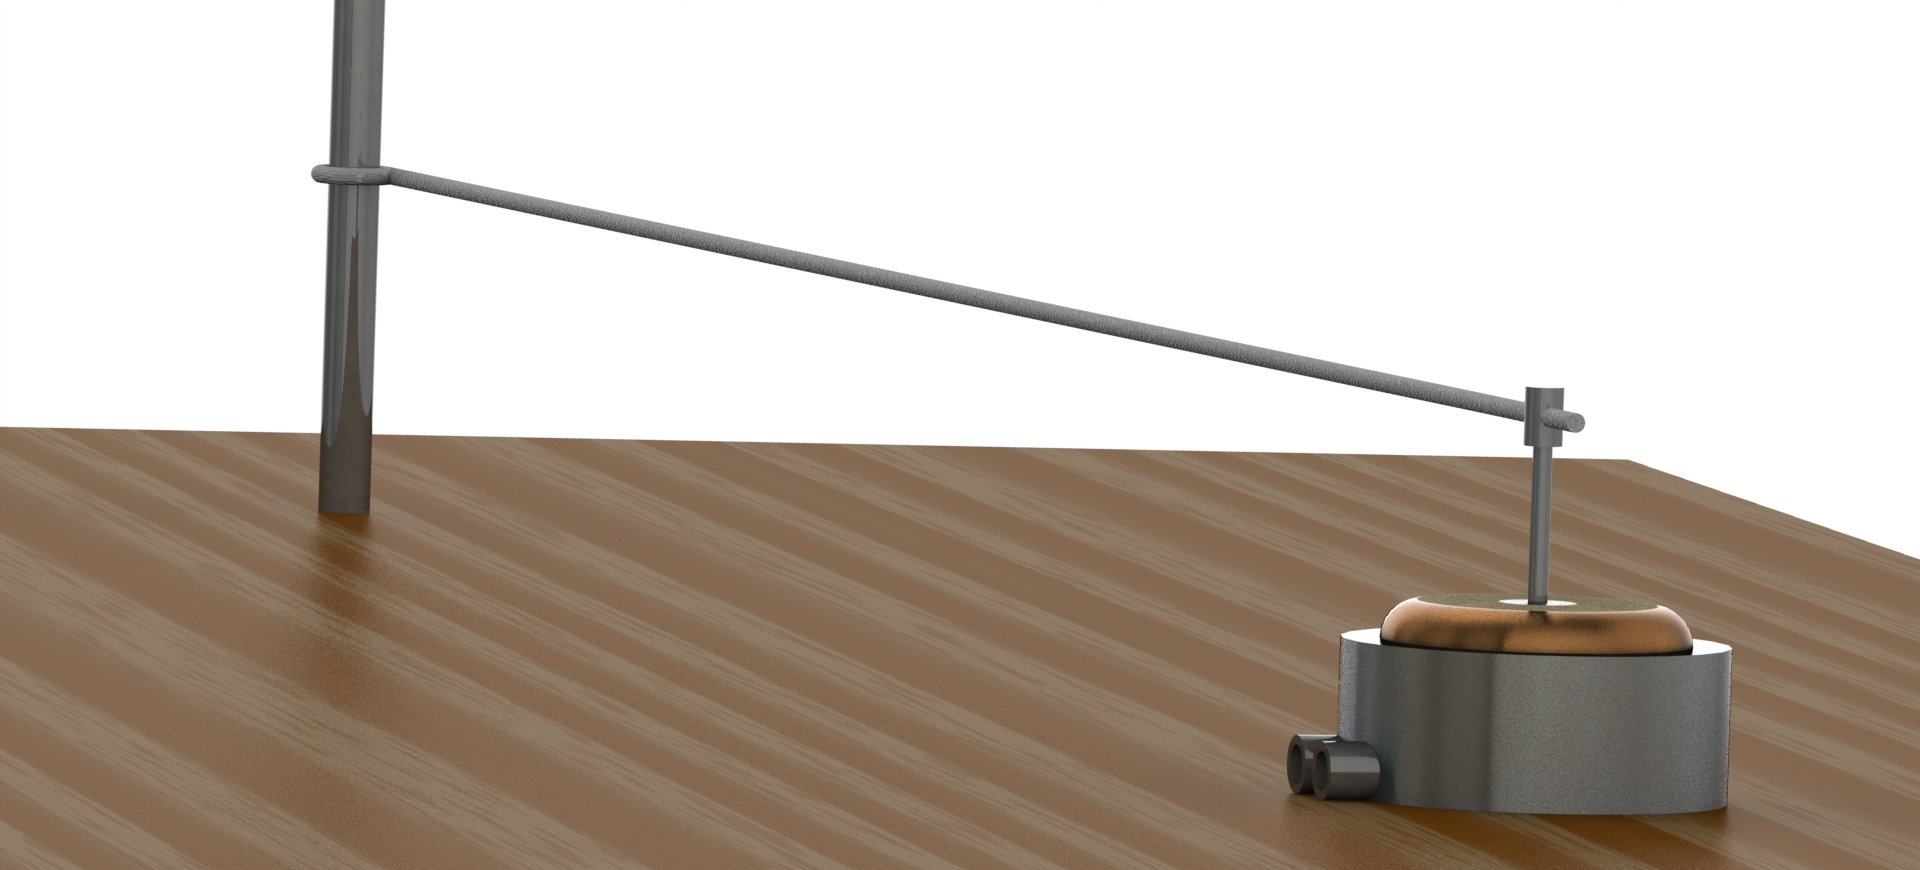
\includegraphics[width=0.5\linewidth]{test.JPG}
	% Sätt vad som ska stå under bilden
	\caption{En testbild}
	% Vilken label du vill använda för att referera till bilden i texten
	\label{fig:test}
\end{figure}

Sedan går det att referera till bilden utan att hålla reda på vilket nummer den har, genom att använda kommandot \textbackslash ref\{figurlabel\}, t.ex.
i figur \ref{fig:test} går det att se en testbild.

\subsection{tabeller}
Tabeller är lite klurigare, man måste säga hur stora de är. För att referera till tabellen används samma sak som till figurer, t.ex. tabell \ref{tab:tabelldata} innehåller data

% Starta en tabellenvironment
\begin{table}[H]
	% Få den centrerad
	\centering
	% Vad som ska stå över den
	\caption{datatabell}
	% Vad man ska referera till
	\label{tab:tabelldata}
	% Starta själva tabellen, de andra paret måsvingar innehåller kolumnerna, med | som linjeavskärmare
	% l betyder att texten läggs till vänster
	% c betyder att texten läggs centrerat
	% r betyder att texten sätts till höger
	\begin{tabular}{|l|c|r|}
% Radlinje
\hline
% Kolumnerna bryts med ett &-tecken, en radbrytning till nästa kolumn är \\
\textbf{1} & \textbf{2} &  \textbf{3} \\
\hline
\hline
data & mer data & ännu mer data \\
\hline
1,23 & 3,54 & 43,65 \\
\hline 
	\end{tabular}
\end{table}

\section{Resultat}

Vilket resultat har uppnåtts.

\section{Diskussion}

Diskutera det som har gjorts, felkällor, eller annat intressant som kan diskuteras från resultaten.

\section{Slutsatser}

Vilka slutsatser kan man dra utifrån resultaten.

% Skriv ut alla referenser och källor som har använts i rapporten
\newpage
\printbibliography

\end{document}
